% Options for packages loaded elsewhere
\PassOptionsToPackage{unicode}{hyperref}
\PassOptionsToPackage{hyphens}{url}
\documentclass[
]{article}
\usepackage{xcolor}
\usepackage[top=3.3cm,bottom=2.5cm,left=2.5cm,right=2.5cm,headheight=1.4cm,headsep=0.7cm]{geometry}
\usepackage{amsmath,amssymb}
\setcounter{secnumdepth}{-\maxdimen} % remove section numbering
\usepackage{iftex}
\ifPDFTeX
  \usepackage[T1]{fontenc}
  \usepackage[utf8]{inputenc}
  \usepackage{textcomp} % provide euro and other symbols
\else % if luatex or xetex
  \usepackage{unicode-math} % this also loads fontspec
  \defaultfontfeatures{Scale=MatchLowercase}
  \defaultfontfeatures[\rmfamily]{Ligatures=TeX,Scale=1}
\fi
\usepackage{lmodern}
\ifPDFTeX\else
  % xetex/luatex font selection
\fi
% Use upquote if available, for straight quotes in verbatim environments
\IfFileExists{upquote.sty}{\usepackage{upquote}}{}
\IfFileExists{microtype.sty}{% use microtype if available
  \usepackage[]{microtype}
  \UseMicrotypeSet[protrusion]{basicmath} % disable protrusion for tt fonts
}{}
\makeatletter
\@ifundefined{KOMAClassName}{% if non-KOMA class
  \IfFileExists{parskip.sty}{%
    \usepackage{parskip}
  }{% else
    \setlength{\parindent}{0pt}
    \setlength{\parskip}{6pt plus 2pt minus 1pt}}
}{% if KOMA class
  \KOMAoptions{parskip=half}}
\makeatother
\usepackage{color}
\usepackage{fancyvrb}
\newcommand{\VerbBar}{|}
\newcommand{\VERB}{\Verb[commandchars=\\\{\}]}
\DefineVerbatimEnvironment{Highlighting}{Verbatim}{commandchars=\\\{\}}
% Add ',fontsize=\small' for more characters per line
\usepackage{framed}
\definecolor{shadecolor}{RGB}{248,248,248}
\newenvironment{Shaded}{\begin{snugshade}}{\end{snugshade}}
\newcommand{\AlertTok}[1]{\textcolor[rgb]{0.94,0.16,0.16}{#1}}
\newcommand{\AnnotationTok}[1]{\textcolor[rgb]{0.56,0.35,0.01}{\textbf{\textit{#1}}}}
\newcommand{\AttributeTok}[1]{\textcolor[rgb]{0.13,0.29,0.53}{#1}}
\newcommand{\BaseNTok}[1]{\textcolor[rgb]{0.00,0.00,0.81}{#1}}
\newcommand{\BuiltInTok}[1]{#1}
\newcommand{\CharTok}[1]{\textcolor[rgb]{0.31,0.60,0.02}{#1}}
\newcommand{\CommentTok}[1]{\textcolor[rgb]{0.56,0.35,0.01}{\textit{#1}}}
\newcommand{\CommentVarTok}[1]{\textcolor[rgb]{0.56,0.35,0.01}{\textbf{\textit{#1}}}}
\newcommand{\ConstantTok}[1]{\textcolor[rgb]{0.56,0.35,0.01}{#1}}
\newcommand{\ControlFlowTok}[1]{\textcolor[rgb]{0.13,0.29,0.53}{\textbf{#1}}}
\newcommand{\DataTypeTok}[1]{\textcolor[rgb]{0.13,0.29,0.53}{#1}}
\newcommand{\DecValTok}[1]{\textcolor[rgb]{0.00,0.00,0.81}{#1}}
\newcommand{\DocumentationTok}[1]{\textcolor[rgb]{0.56,0.35,0.01}{\textbf{\textit{#1}}}}
\newcommand{\ErrorTok}[1]{\textcolor[rgb]{0.64,0.00,0.00}{\textbf{#1}}}
\newcommand{\ExtensionTok}[1]{#1}
\newcommand{\FloatTok}[1]{\textcolor[rgb]{0.00,0.00,0.81}{#1}}
\newcommand{\FunctionTok}[1]{\textcolor[rgb]{0.13,0.29,0.53}{\textbf{#1}}}
\newcommand{\ImportTok}[1]{#1}
\newcommand{\InformationTok}[1]{\textcolor[rgb]{0.56,0.35,0.01}{\textbf{\textit{#1}}}}
\newcommand{\KeywordTok}[1]{\textcolor[rgb]{0.13,0.29,0.53}{\textbf{#1}}}
\newcommand{\NormalTok}[1]{#1}
\newcommand{\OperatorTok}[1]{\textcolor[rgb]{0.81,0.36,0.00}{\textbf{#1}}}
\newcommand{\OtherTok}[1]{\textcolor[rgb]{0.56,0.35,0.01}{#1}}
\newcommand{\PreprocessorTok}[1]{\textcolor[rgb]{0.56,0.35,0.01}{\textit{#1}}}
\newcommand{\RegionMarkerTok}[1]{#1}
\newcommand{\SpecialCharTok}[1]{\textcolor[rgb]{0.81,0.36,0.00}{\textbf{#1}}}
\newcommand{\SpecialStringTok}[1]{\textcolor[rgb]{0.31,0.60,0.02}{#1}}
\newcommand{\StringTok}[1]{\textcolor[rgb]{0.31,0.60,0.02}{#1}}
\newcommand{\VariableTok}[1]{\textcolor[rgb]{0.00,0.00,0.00}{#1}}
\newcommand{\VerbatimStringTok}[1]{\textcolor[rgb]{0.31,0.60,0.02}{#1}}
\newcommand{\WarningTok}[1]{\textcolor[rgb]{0.56,0.35,0.01}{\textbf{\textit{#1}}}}
\usepackage{graphicx}
\makeatletter
\newsavebox\pandoc@box
\newcommand*\pandocbounded[1]{% scales image to fit in text height/width
  \sbox\pandoc@box{#1}%
  \Gscale@div\@tempa{\textheight}{\dimexpr\ht\pandoc@box+\dp\pandoc@box\relax}%
  \Gscale@div\@tempb{\linewidth}{\wd\pandoc@box}%
  \ifdim\@tempb\p@<\@tempa\p@\let\@tempa\@tempb\fi% select the smaller of both
  \ifdim\@tempa\p@<\p@\scalebox{\@tempa}{\usebox\pandoc@box}%
  \else\usebox{\pandoc@box}%
  \fi%
}
% Set default figure placement to htbp
\def\fps@figure{htbp}
\makeatother
\setlength{\emergencystretch}{3em} % prevent overfull lines
\providecommand{\tightlist}{%
  \setlength{\itemsep}{0pt}\setlength{\parskip}{0pt}}
\usepackage{fancyhdr}
\usepackage{lastpage}
\definecolor{grisur}{HTML}{808080}
\pagestyle{fancy}
\fancyhf{}
\fancyhead[L]{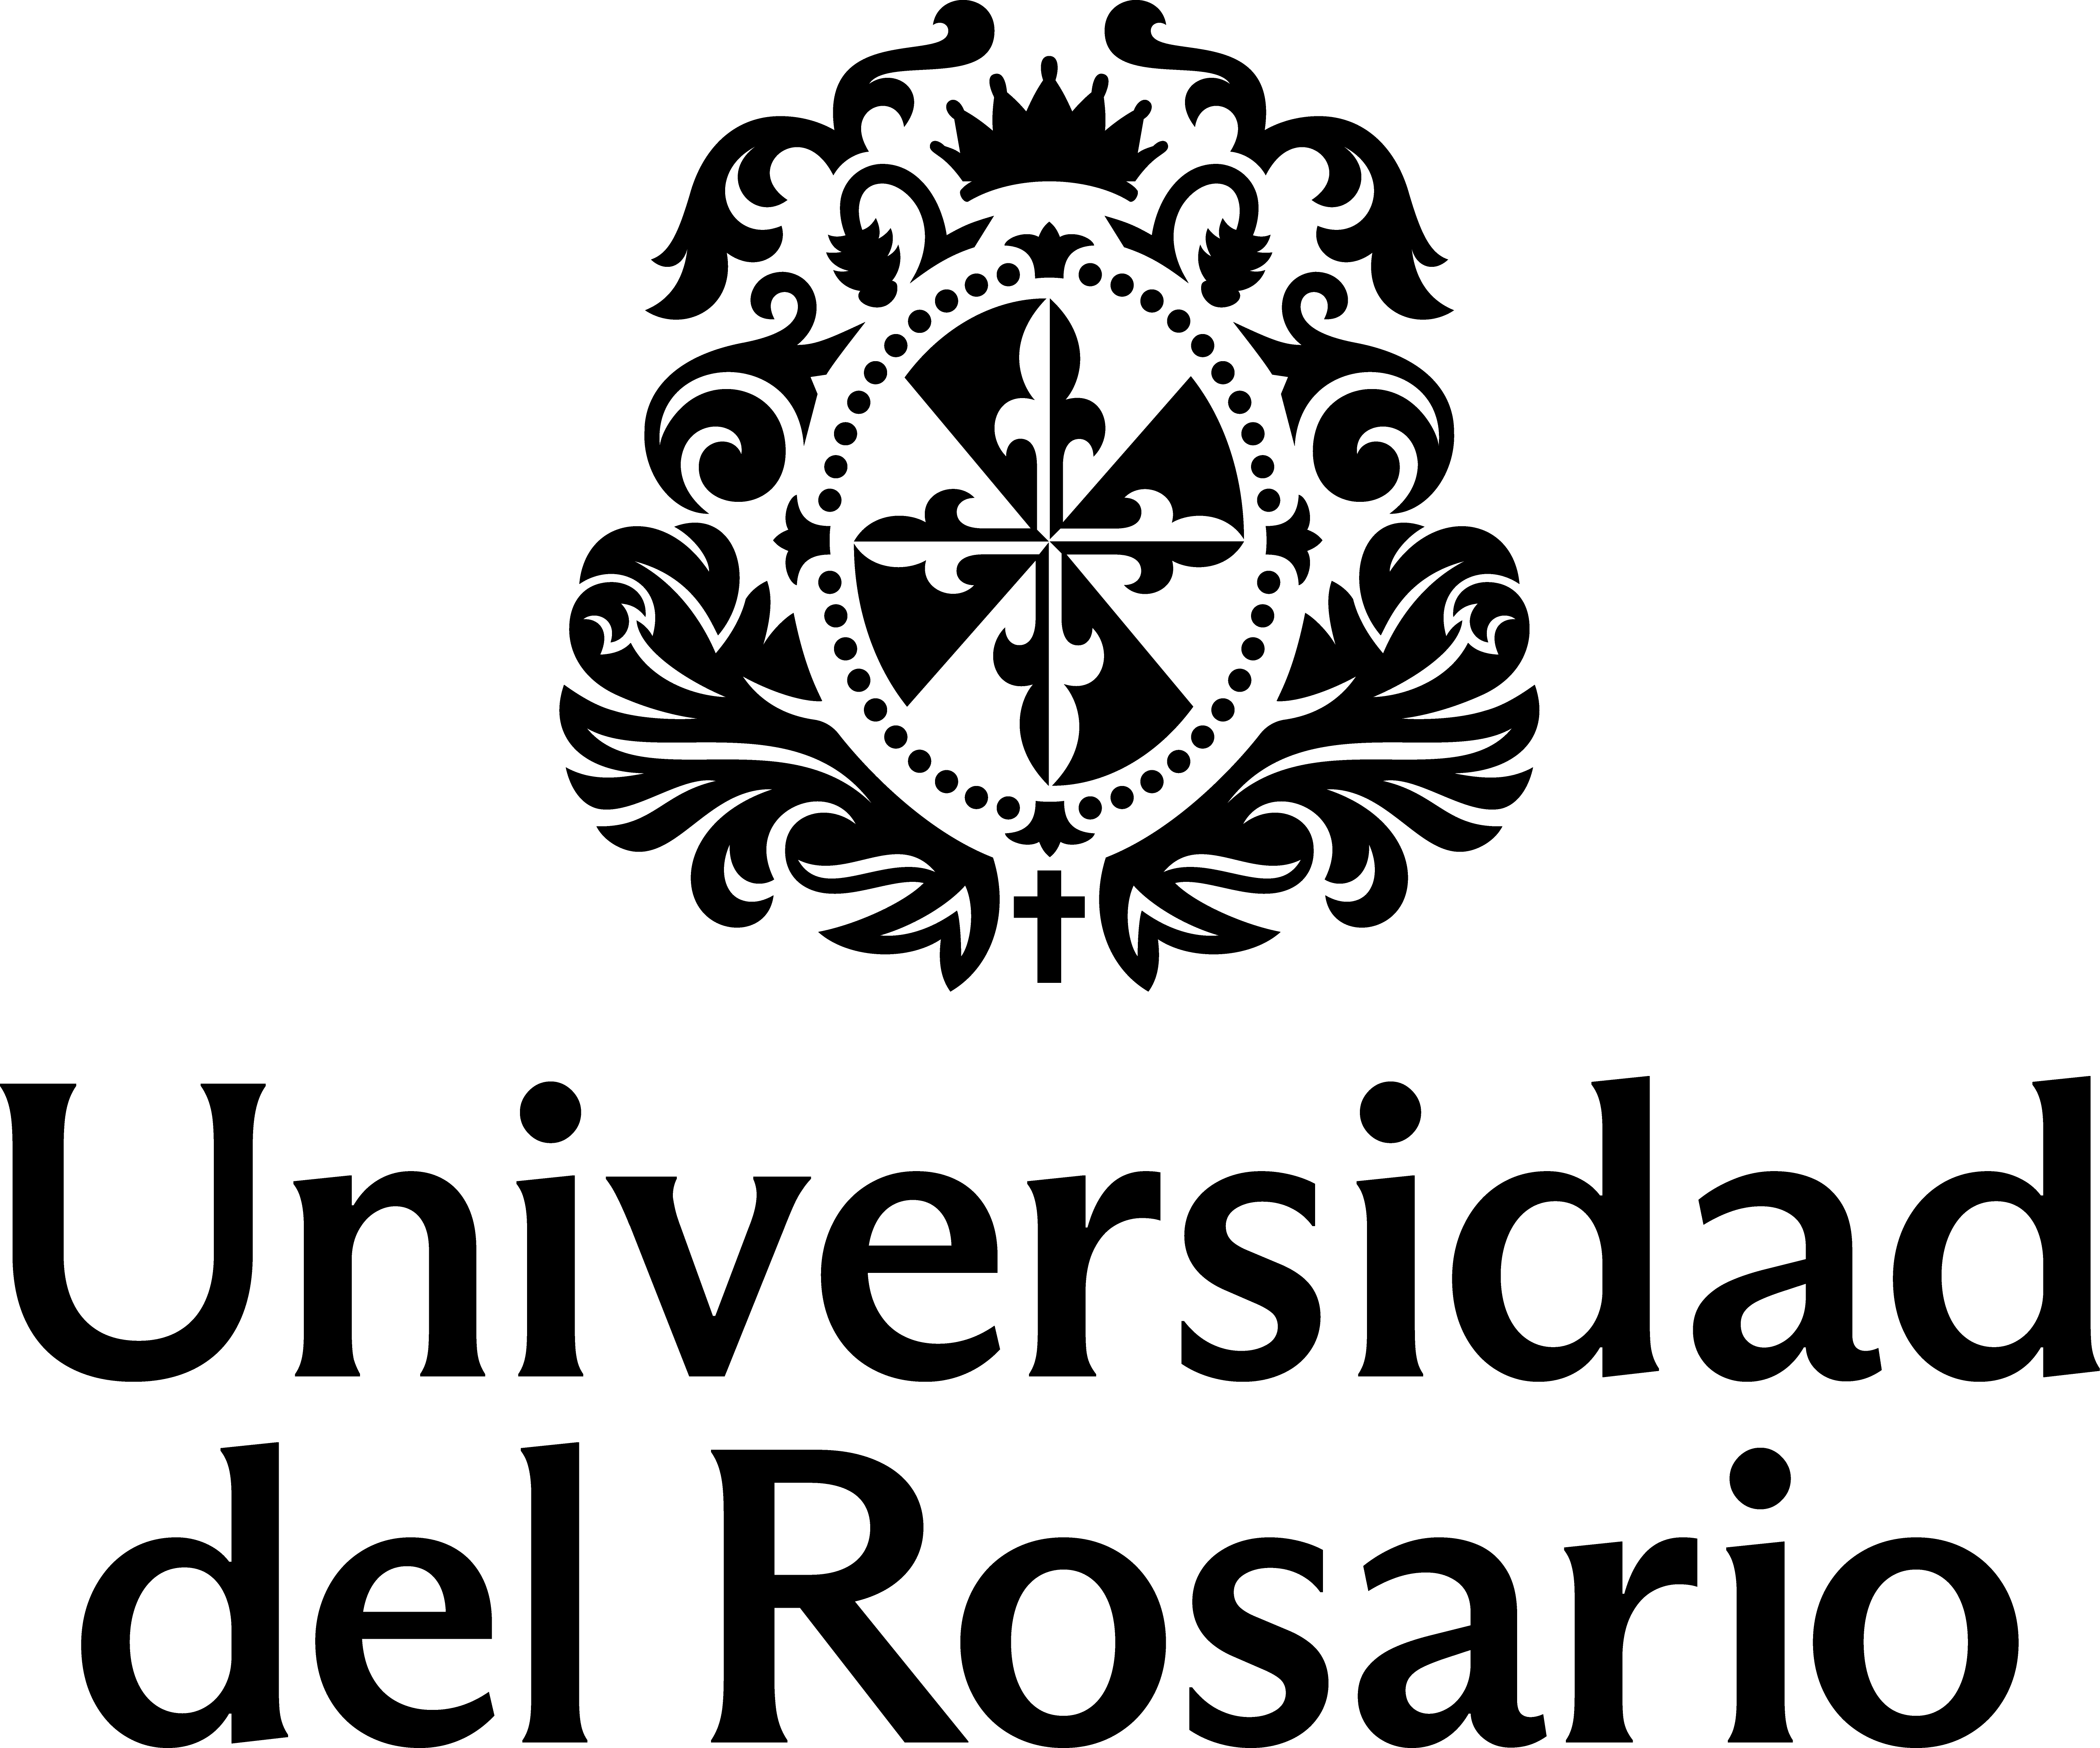
\includegraphics[height=1.2cm]{logo_ur.png}}
\fancyhead[R]{\color{grisur}\small Escuela de Ciencias e Ingeniería\\ Análisis Estadístico de Datos}
\renewcommand{\headrulewidth}{0pt}
\fancyfoot[L]{\color{grisur}\footnotesize Universidad del Rosario · Bogotá D.C., Colombia}
\fancyfoot[R]{\color{grisur}\footnotesize Página \thepage\ de \pageref{LastPage}}
\renewcommand{\footrule}{{\color{grisur}\hrule width\headwidth height 0.4pt}\vspace{4pt}}
\makeatletter\let\ps@plain\ps@fancy\makeatother
\usepackage{bookmark}
\IfFileExists{xurl.sty}{\usepackage{xurl}}{} % add URL line breaks if available
\urlstyle{same}
\hypersetup{
  pdftitle={Análisis Estadístico de Datos - Taller 03},
  pdfauthor={Adriana Porras, Alejandra Niño, Bayron Morales, Juliana Cárdenas},
  hidelinks,
  pdfcreator={LaTeX via pandoc}}

\title{Análisis Estadístico de Datos - Taller 03}
\author{Adriana Porras, Alejandra Niño, Bayron Morales, Juliana
Cárdenas}
\date{}

\begin{document}
\maketitle

\begin{Shaded}
\begin{Highlighting}[]
\CommentTok{\# Instalación de librerias en caso de no tenerlas}
\CommentTok{\# install.packages("tidyverse")}
\CommentTok{\# install.packages("plotly")}
\CommentTok{\# install.packages("MASS")}
\CommentTok{\# install.packages("psych")}
\CommentTok{\# install.packages("factoextra")}
\CommentTok{\# install.packages("GGally")}
\CommentTok{\# install.packages("dplyr")}
\CommentTok{\#install.packages("downcute")}

\CommentTok{\# Ejecución de librerias}
\FunctionTok{library}\NormalTok{(tidyverse)}
\CommentTok{\# library(downcute)}
\CommentTok{\#library(plotly)}
\CommentTok{\#library(MASS)}
\CommentTok{\#library(psych)}
\CommentTok{\#library(tidyverse)}
\CommentTok{\#library(factoextra)}
\FunctionTok{library}\NormalTok{(GGally)}
\CommentTok{\#library(dplyr)}
\end{Highlighting}
\end{Shaded}

\begin{Shaded}
\begin{Highlighting}[]
\CommentTok{\# Colores usados en todos los gráficos del taller}
\NormalTok{rojo        }\OtherTok{\textless{}{-}} \StringTok{"\#DA0921"}
\NormalTok{rojo\_oscuro }\OtherTok{\textless{}{-}} \StringTok{"\#950606"}
\end{Highlighting}
\end{Shaded}

\begin{center}\rule{0.5\linewidth}{0.5pt}\end{center}

\subsection{Modelo de Regresión Lineal
Múltiple}\label{modelo-de-regresiuxf3n-lineal-muxfaltiple}

\subsection{EIA data}\label{eia-data}

U.S. Energy Information Administration
(\href{https://www.eia.gov/}{EIA}) es una organización que se encarga de
recopilar, analizar y difundir información energética de manera
independiente e imparcial para promover la formulación de políticas
sólidas, mercados eficientes y la comprensión pública de la energía y su
interacción con la economía y el medio ambiente. Los datos que
trabajaremos a continuación corresponden a la extracción de diferentes
variables relacionadas con energías renovables y combustibles fósiles,
las UE son 111 países de todos los continentes del mundo, seleccionados
para fines académicos por ser aquellos países que presentan mayor
cantidad de información de análisis. Adicionalmente, se han incluido
variables relacionadas al Producto interno Bruto de cada país para el
año 2014 (GDP\_USD y GDP\_per\_capita), así como la población de cada
país a final de ese año.

El objetivo de este análisis es encontrar estructuras de correlación de
tipo lineal entre la generación de combustibles fósiles y de energías
renovables con el PIB de cada país, entendiendo que nuestras variables
explicativas solamente son una parte del total del PIB. Trabaje los
ejercicios 1 a 5 con los datos manipulados a continuación:

\begin{Shaded}
\begin{Highlighting}[]
\NormalTok{datos }\OtherTok{=} \FunctionTok{read.csv}\NormalTok{(}\StringTok{"datos\_taller\_03.csv"}\NormalTok{, }\AttributeTok{sep=}\StringTok{";"}\NormalTok{) }\SpecialCharTok{\%\textgreater{}\%} \FunctionTok{as\_tibble}\NormalTok{() }\SpecialCharTok{\%\textgreater{}\%} 
\NormalTok{  dplyr}\SpecialCharTok{::}\FunctionTok{filter}\NormalTok{(}\SpecialCharTok{!}\NormalTok{Country }\SpecialCharTok{\%in\%} \FunctionTok{c}\NormalTok{(}\StringTok{\textquotesingle{}UnitedStates\textquotesingle{}}\NormalTok{,}\StringTok{\textquotesingle{}China\textquotesingle{}}\NormalTok{,}\StringTok{\textquotesingle{}SaudiArabia\textquotesingle{}}\NormalTok{,}\StringTok{\textquotesingle{}Russia\textquotesingle{}}\NormalTok{)) }\SpecialCharTok{\%\textgreater{}\%} 
\NormalTok{  dplyr}\SpecialCharTok{::}\FunctionTok{select}\NormalTok{(}\FunctionTok{c}\NormalTok{(}\StringTok{"GDP\_USD"}\NormalTok{,}\StringTok{"Population"}\NormalTok{,}\StringTok{"Solar\_electricity\_net\_generation\_BKWH"}\NormalTok{,}\StringTok{"Wind\_electricity\_net\_generation\_BKWH"}\NormalTok{)) }\SpecialCharTok{\%\textgreater{}\%}
\NormalTok{  dplyr}\SpecialCharTok{::}\FunctionTok{filter}\NormalTok{(Solar\_electricity\_net\_generation\_BKWH }\SpecialCharTok{\textgreater{}}\DecValTok{0} \SpecialCharTok{\&}\NormalTok{ Wind\_electricity\_net\_generation\_BKWH}\SpecialCharTok{\textgreater{}}\DecValTok{0}\NormalTok{) }\SpecialCharTok{\%\textgreater{}\%} 
\NormalTok{  dplyr}\SpecialCharTok{::}\FunctionTok{mutate}\NormalTok{(}\AttributeTok{GDP\_USD\_PER\_CAPITA =}\NormalTok{ GDP\_USD}\SpecialCharTok{/}\NormalTok{Population) }\SpecialCharTok{\%\textgreater{}\%} 
\NormalTok{  dplyr}\SpecialCharTok{::}\FunctionTok{select}\NormalTok{(}\SpecialCharTok{{-}}\FunctionTok{c}\NormalTok{(}\StringTok{\textquotesingle{}GDP\_USD\textquotesingle{}}\NormalTok{,}\StringTok{\textquotesingle{}Population\textquotesingle{}}\NormalTok{)) }

\CommentTok{\# Revisar tamaño de la base: 28 países y 3 variables}
\FunctionTok{dim}\NormalTok{(datos)}
\end{Highlighting}
\end{Shaded}

\begin{verbatim}
## [1] 28  3
\end{verbatim}

\noindent\textbf{Pregunta 1. Mediante la función `GGally::ggpairs`, grafique los diagramas de dispersión bivariados para el conjunto de datos. ¿Qué tipo de relación observa entre cada par de variables? ¿Visualmente considera que las variables Solar\_electricity\_net\_generation\_BKWH y Wind\_electricity\_net\_generation\_BKWH presentan varianza constante, (también llamada homoscedasticidad) a través de los valores de la variable GDP\_USD\_PER\_CAPITA?}

\begin{Shaded}
\begin{Highlighting}[]
\FunctionTok{ggpairs}\NormalTok{(datos)}
\end{Highlighting}
\end{Shaded}

\begin{center}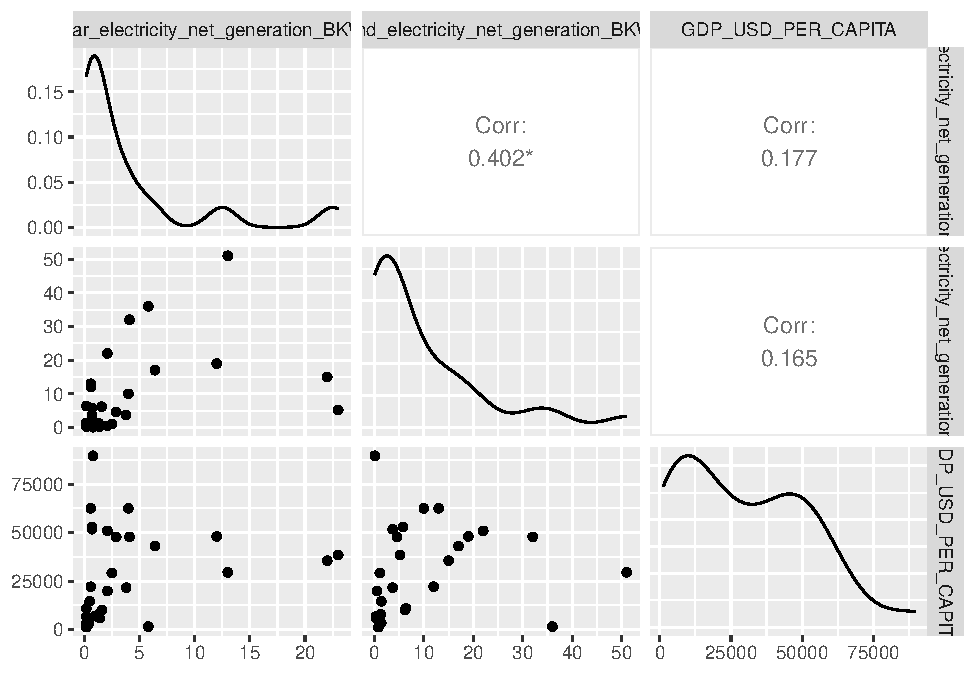
\includegraphics[width=1\linewidth]{Taller-03_files/figure-latex/Graf_dispersión-1} \end{center}

\ldots.

\noindent\textbf{Pregunta 2. Para explicar el PIB per capita (GDP\_USD\_PER\_CAPITA) a través de las variables en la tabla `datos` de manera simultánea, ajuste un modelo de regresión con todas las variables explicativas e interprete la salida del mismo con la ayuda de la función `summary()`. ¿Cómo interpretaría los coeficientes estimados del modelo? ¿Cuál variable parece ser más importante para explicar el GDP\_USD\_PER\_CAPITA?}

\begin{Shaded}
\begin{Highlighting}[]
\NormalTok{mod }\OtherTok{\textless{}{-}} \FunctionTok{lm}\NormalTok{(GDP\_USD\_PER\_CAPITA }\SpecialCharTok{\textasciitilde{}} 
\NormalTok{            Solar\_electricity\_net\_generation\_BKWH }\SpecialCharTok{+} 
\NormalTok{            Wind\_electricity\_net\_generation\_BKWH, }
          \AttributeTok{data=}\NormalTok{datos)}

\FunctionTok{summary}\NormalTok{(mod)}
\end{Highlighting}
\end{Shaded}

\begin{verbatim}
## 
## Call:
## lm(formula = GDP_USD_PER_CAPITA ~ Solar_electricity_net_generation_BKWH + 
##     Wind_electricity_net_generation_BKWH, data = datos)
## 
## Residuals:
##    Min     1Q Median     3Q    Max 
## -34248 -18556  -6296  15218  63845 
## 
## Coefficients:
##                                       Estimate Std. Error t value Pr(>|t|)    
## (Intercept)                            25415.4     5995.9   4.239 0.000268 ***
## Solar_electricity_net_generation_BKWH    504.1      815.7   0.618 0.542158    
## Wind_electricity_net_generation_BKWH     207.8      399.0   0.521 0.606980    
## ---
## Signif. codes:  0 '***' 0.001 '**' 0.01 '*' 0.05 '.' 0.1 ' ' 1
## 
## Residual standard error: 23810 on 25 degrees of freedom
## Multiple R-squared:  0.04173,    Adjusted R-squared:  -0.03493 
## F-statistic: 0.5443 on 2 and 25 DF,  p-value: 0.587
\end{verbatim}

\ldots{}

\noindent\textbf{Pregunta 3. Según la salida de `summary()` anterior, ¿cuál es el valor del estadístico F del modelo?. Dado su valor y el valor p asociado del modelo, ¿son estas variables en conjunto relevantes desde el punto de vista estadístico para explicar el PIB?.}

\ldots{}

\noindent\textbackslash textbf\{Pregunta 4. A través de los gráficos
asociados al modelo obtenidos con la función \texttt{plot()}, mencione
respecto a los supuestos de:

\begin{itemize}
\item
  Normalidad de los errores del modelo.
\item
  Varianza constante.
\end{itemize}

¿Parece el modelo seguir los dos supuestos mencionados?\}

\begin{Shaded}
\begin{Highlighting}[]
\FunctionTok{par}\NormalTok{(}\AttributeTok{mfrow=}\FunctionTok{c}\NormalTok{(}\DecValTok{2}\NormalTok{,}\DecValTok{2}\NormalTok{))}
\FunctionTok{plot}\NormalTok{(mod)}
\end{Highlighting}
\end{Shaded}

\begin{center}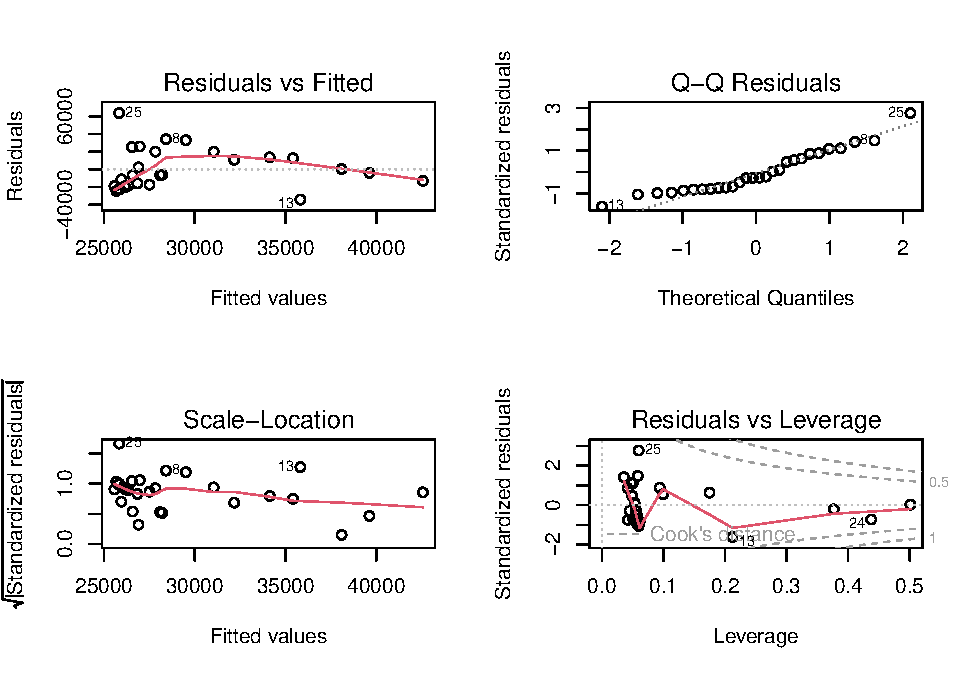
\includegraphics[width=1\linewidth]{Taller-03_files/figure-latex/unnamed-chunk-2-1} \end{center}

\noindent\textbf{Pregunta 5. Estime ahora un modelo de regresión lineal múltiple, pero esta vez realice una transformación de logaritmo sobre la variable de respuesta `log(GDP\_USD\_PER\_CAPITA)`. ¿Qué pasa ahora con el modelo cuando realizamos esta transformación? ¿Cuál modelo presenta residuales más cercanos a la distribución normal?}

\ldots{}

\begin{center}\rule{0.5\linewidth}{0.5pt}\end{center}

\subsection{Anova}\label{anova}

En el conjunto de datos \texttt{turbinas\textbackslash{}\_prod.csv}
cuenta con la producción mensual promedio de 5 turbinas eólicas ubicadas
en la Guajira. Esta información se tiene por un total de 12 meses para
cada turbina y la medición esta dada en MWh. Se busca determinar si
existen diferencias significativas entre la producción promedio de
energía de las turbinas.

\begin{Shaded}
\begin{Highlighting}[]
\NormalTok{datos2 }\OtherTok{\textless{}{-}} \FunctionTok{read.csv}\NormalTok{(}\StringTok{"turbinas\_prod.csv"}\NormalTok{, }\AttributeTok{sep=}\StringTok{","}\NormalTok{)}
\end{Highlighting}
\end{Shaded}

\noindent\textbf{Pregunta 6. Realice el boxplot de producción para las diferentes turbinas y determine visualmente si observa diferencias en la producción de energía de las 5 turbinas. ¿Parece haber varianza constante en las observaciones de las turbinas?}

\begin{Shaded}
\begin{Highlighting}[]
\CommentTok{\# Crear una función para crear boxplot}

\NormalTok{boxplot\_estadisticos }\OtherTok{\textless{}{-}} \ControlFlowTok{function}\NormalTok{(data2, variable, titulo, subtitulo, etiqueta\_x) \{}
  
\NormalTok{  valores }\OtherTok{\textless{}{-}}\NormalTok{ data2[[variable]]}
  
\NormalTok{  estadisticos }\OtherTok{\textless{}{-}} \FunctionTok{boxplot.stats}\NormalTok{(valores)}\SpecialCharTok{$}\NormalTok{stats}
  
\NormalTok{  etiquetas }\OtherTok{\textless{}{-}} \FunctionTok{data.frame}\NormalTok{(}
    \AttributeTok{x =} \FunctionTok{as.numeric}\NormalTok{(estadisticos),}
    \AttributeTok{y =} \FunctionTok{c}\NormalTok{(}\FloatTok{1.20}\NormalTok{, }\FloatTok{1.30}\NormalTok{, }\FloatTok{1.40}\NormalTok{, }\FloatTok{1.50}\NormalTok{, }\FloatTok{1.60}\NormalTok{),}
    \AttributeTok{etiqueta =} \FunctionTok{c}\NormalTok{(}
      \FunctionTok{paste0}\NormalTok{(}\StringTok{"Bigote inf.: "}\NormalTok{, }\FunctionTok{round}\NormalTok{(estadisticos[}\DecValTok{1}\NormalTok{], }\DecValTok{1}\NormalTok{)),}
      \FunctionTok{paste0}\NormalTok{(}\StringTok{"Q1: "}\NormalTok{, }\FunctionTok{round}\NormalTok{(estadisticos[}\DecValTok{2}\NormalTok{], }\DecValTok{1}\NormalTok{)),}
      \FunctionTok{paste0}\NormalTok{(}\StringTok{"Q2: "}\NormalTok{, }\FunctionTok{round}\NormalTok{(estadisticos[}\DecValTok{3}\NormalTok{], }\DecValTok{1}\NormalTok{)),}
      \FunctionTok{paste0}\NormalTok{(}\StringTok{"Q3: "}\NormalTok{, }\FunctionTok{round}\NormalTok{(estadisticos[}\DecValTok{4}\NormalTok{], }\DecValTok{1}\NormalTok{)),}
      \FunctionTok{paste0}\NormalTok{(}\StringTok{"Bigote sup.: "}\NormalTok{, }\FunctionTok{round}\NormalTok{(estadisticos[}\DecValTok{5}\NormalTok{], }\DecValTok{1}\NormalTok{))))}
  
  \FunctionTok{ggplot}\NormalTok{(data2, }\FunctionTok{aes}\NormalTok{(}\AttributeTok{x =}\NormalTok{ .data[[variable]], }\AttributeTok{y =} \DecValTok{1}\NormalTok{)) }\SpecialCharTok{+}
    
    \FunctionTok{geom\_boxplot}\NormalTok{(}
      \AttributeTok{fill =}\NormalTok{ rojo,}
      \AttributeTok{color =}\NormalTok{ rojo\_oscuro,}
      \AttributeTok{width =} \FloatTok{0.35}\NormalTok{) }\SpecialCharTok{+}
    
    \FunctionTok{geom\_segment}\NormalTok{(}
      \AttributeTok{data =}\NormalTok{ etiquetas,}
      \FunctionTok{aes}\NormalTok{(}
        \AttributeTok{x =}\NormalTok{ x,}
        \AttributeTok{xend =}\NormalTok{ x,}
        \AttributeTok{y =} \FloatTok{0.82}\NormalTok{,}
        \AttributeTok{yend =}\NormalTok{ y}
\NormalTok{      ),}
      \AttributeTok{color =}\NormalTok{ rojo\_oscuro,}
      \AttributeTok{linewidth =} \FloatTok{0.5}\NormalTok{,}
      \AttributeTok{linetype =} \StringTok{"dashed"}\NormalTok{) }\SpecialCharTok{+}
    
    \FunctionTok{geom\_text}\NormalTok{(}
      \AttributeTok{data =}\NormalTok{ etiquetas,}
      \FunctionTok{aes}\NormalTok{(}
        \AttributeTok{x =}\NormalTok{ x,}
        \AttributeTok{y =}\NormalTok{ y,}
        \AttributeTok{label =}\NormalTok{ etiqueta}
\NormalTok{      ),}
      \AttributeTok{hjust =} \SpecialCharTok{{-}}\FloatTok{0.05}\NormalTok{,}
      \AttributeTok{size =} \FloatTok{3.5}\NormalTok{,}
      \AttributeTok{fontface =} \StringTok{"bold"}\NormalTok{,}
      \AttributeTok{color =} \StringTok{"\#950606"}\NormalTok{) }\SpecialCharTok{+}
    
    \FunctionTok{labs}\NormalTok{(}
      \AttributeTok{title =}\NormalTok{ titulo,}
      \AttributeTok{subtitle =}\NormalTok{ subtitulo,}
      \AttributeTok{x =}\NormalTok{ etiqueta\_x,}
      \AttributeTok{y =} \ConstantTok{NULL}\NormalTok{) }\SpecialCharTok{+}
    
    \FunctionTok{theme\_minimal}\NormalTok{() }\SpecialCharTok{+}
    
    \FunctionTok{theme}\NormalTok{(}
      \AttributeTok{plot.title =} \FunctionTok{element\_text}\NormalTok{(}
        \AttributeTok{face =} \StringTok{"bold"}\NormalTok{,}
        \AttributeTok{size =} \DecValTok{14}\NormalTok{,}
        \AttributeTok{hjust =} \FloatTok{0.5}\NormalTok{),}
      \AttributeTok{plot.subtitle =} \FunctionTok{element\_text}\NormalTok{(}
        \AttributeTok{size =} \DecValTok{11}\NormalTok{,}
        \AttributeTok{hjust =} \FloatTok{0.5}\NormalTok{),}
      \AttributeTok{axis.text.y =} \FunctionTok{element\_blank}\NormalTok{(),}
      \AttributeTok{axis.ticks.y =} \FunctionTok{element\_blank}\NormalTok{(),}
      \AttributeTok{axis.title.y =} \FunctionTok{element\_blank}\NormalTok{(),}
      \AttributeTok{axis.title.x =} \FunctionTok{element\_text}\NormalTok{(}\AttributeTok{face =} \StringTok{"bold"}\NormalTok{),}
      \AttributeTok{panel.grid.minor =} \FunctionTok{element\_blank}\NormalTok{(),}
      \AttributeTok{panel.grid.major.y =} \FunctionTok{element\_blank}\NormalTok{())\}}
\end{Highlighting}
\end{Shaded}

\begin{Shaded}
\begin{Highlighting}[]
\FunctionTok{boxplot\_estadisticos}\NormalTok{(}
\NormalTok{ datos2,}
  \StringTok{"T1"}\NormalTok{,}
  \StringTok{"Distribución Turbina 1"}\NormalTok{,}
  \StringTok{"Producción mensual"}\NormalTok{,}
  \StringTok{"Megavatio{-}hora(MWh)"}\NormalTok{)}
\end{Highlighting}
\end{Shaded}

\begin{center}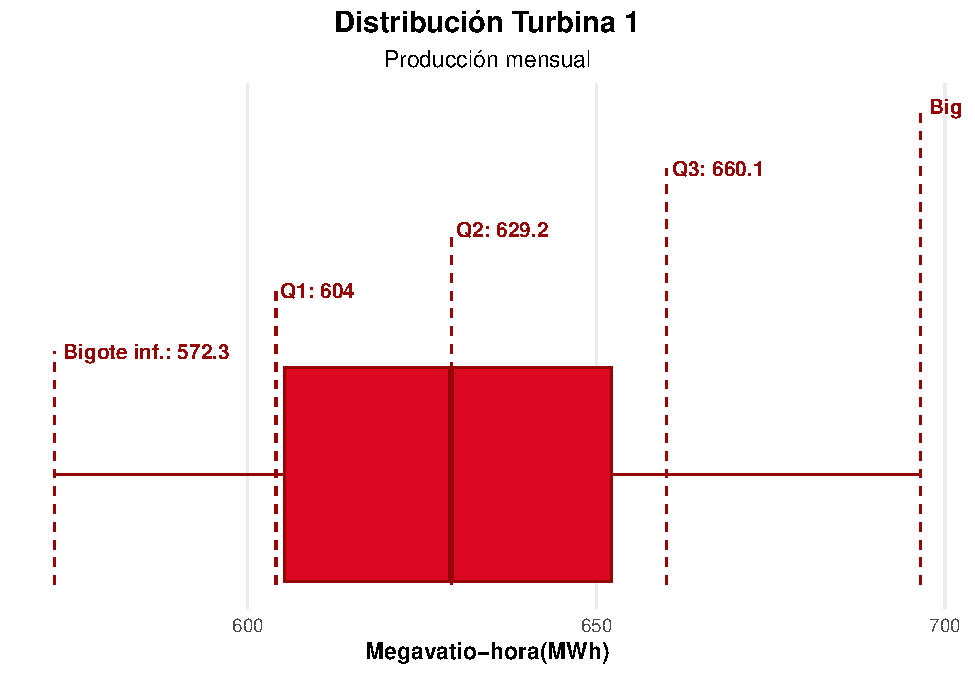
\includegraphics[width=1\linewidth]{Taller-03_files/figure-latex/unnamed-chunk-4-1} \end{center}

\ldots{}

\begin{Shaded}
\begin{Highlighting}[]
\FunctionTok{boxplot\_estadisticos}\NormalTok{(}
\NormalTok{ datos2,}
  \StringTok{"T2"}\NormalTok{,}
  \StringTok{"Distribución Turbina 2"}\NormalTok{,}
  \StringTok{"Producción mensual"}\NormalTok{,}
  \StringTok{"Megavatio{-}hora(MWh)"}\NormalTok{)}
\end{Highlighting}
\end{Shaded}

\begin{center}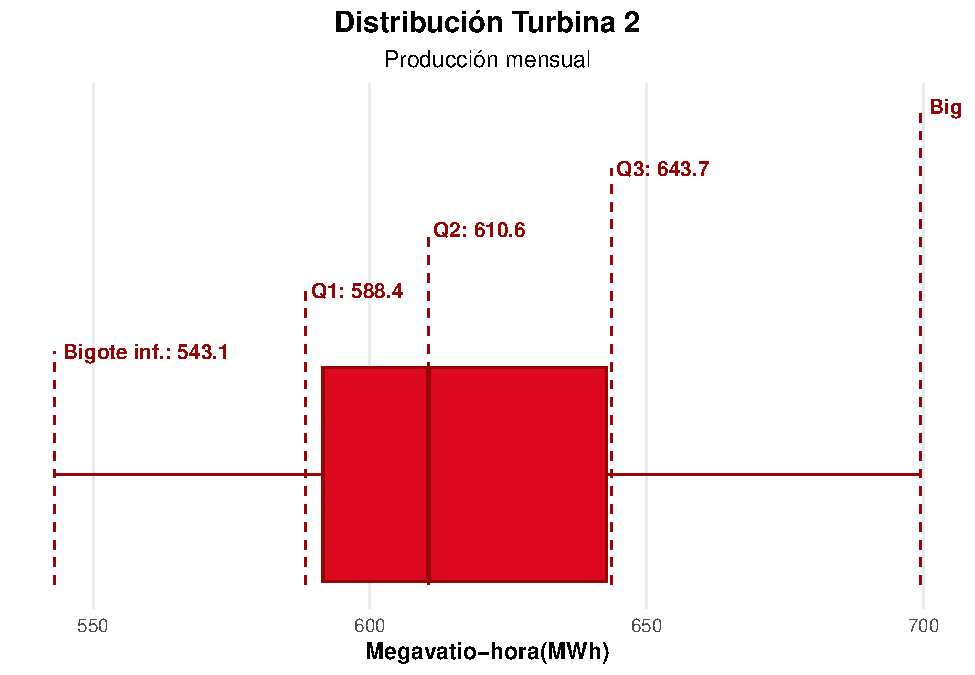
\includegraphics[width=1\linewidth]{Taller-03_files/figure-latex/unnamed-chunk-5-1} \end{center}

\ldots{}

\begin{Shaded}
\begin{Highlighting}[]
\FunctionTok{boxplot\_estadisticos}\NormalTok{(}
\NormalTok{ datos2,}
  \StringTok{"T3"}\NormalTok{,}
  \StringTok{"Distribución Turbina 3"}\NormalTok{,}
  \StringTok{"Producción mensual"}\NormalTok{,}
  \StringTok{"Megavatio{-}hora(MWh)"}\NormalTok{)}
\end{Highlighting}
\end{Shaded}

\begin{center}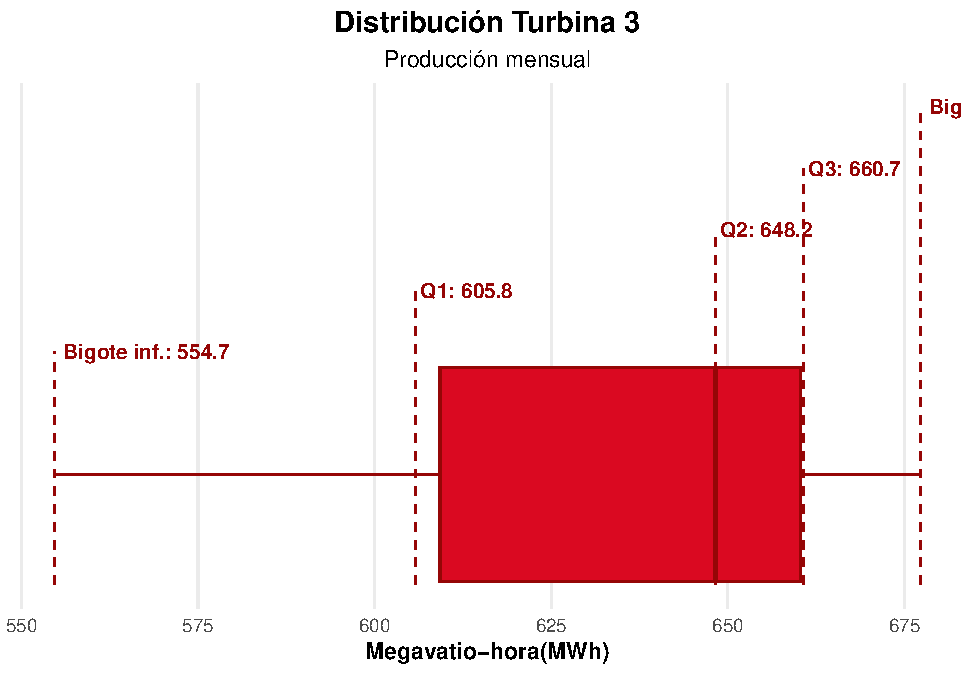
\includegraphics[width=1\linewidth]{Taller-03_files/figure-latex/unnamed-chunk-6-1} \end{center}

\ldots{}

\begin{Shaded}
\begin{Highlighting}[]
\FunctionTok{boxplot\_estadisticos}\NormalTok{(}
\NormalTok{ datos2,}
  \StringTok{"T4"}\NormalTok{,}
  \StringTok{"Distribución Turbina 4"}\NormalTok{,}
  \StringTok{"Producción mensual"}\NormalTok{,}
  \StringTok{"Megavatio{-}hora(MWh)"}\NormalTok{)}
\end{Highlighting}
\end{Shaded}

\begin{center}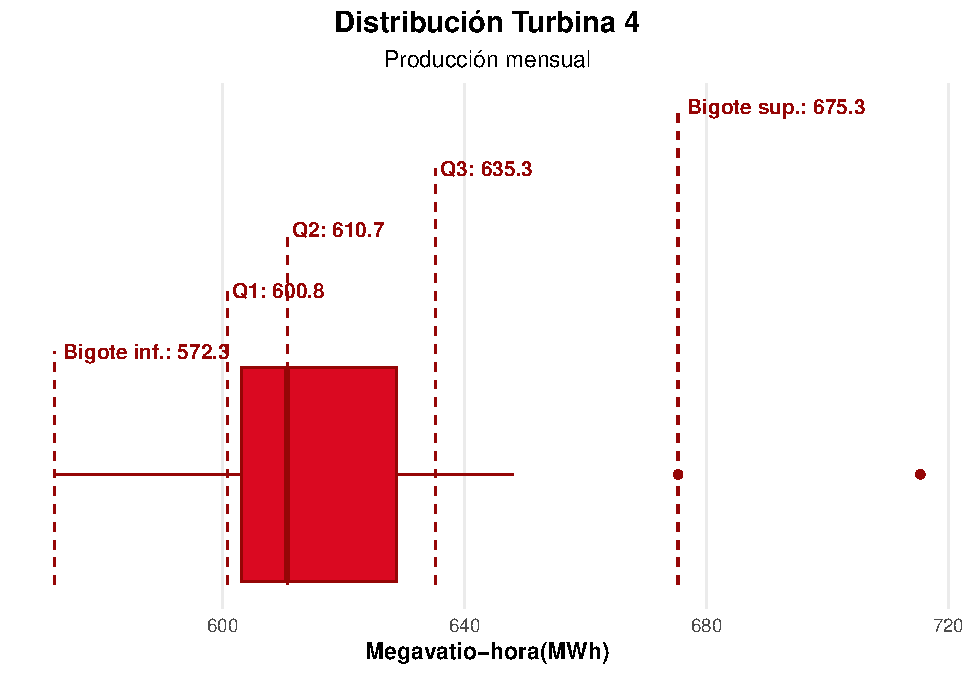
\includegraphics[width=1\linewidth]{Taller-03_files/figure-latex/unnamed-chunk-7-1} \end{center}

\ldots{}

\begin{Shaded}
\begin{Highlighting}[]
\FunctionTok{boxplot\_estadisticos}\NormalTok{(}
\NormalTok{ datos2,}
  \StringTok{"T5"}\NormalTok{,}
  \StringTok{"Distribución Turbina 5"}\NormalTok{,}
  \StringTok{"Producción mensual"}\NormalTok{,}
  \StringTok{"Megavatio{-}hora(MWh)"}\NormalTok{)}
\end{Highlighting}
\end{Shaded}

\begin{center}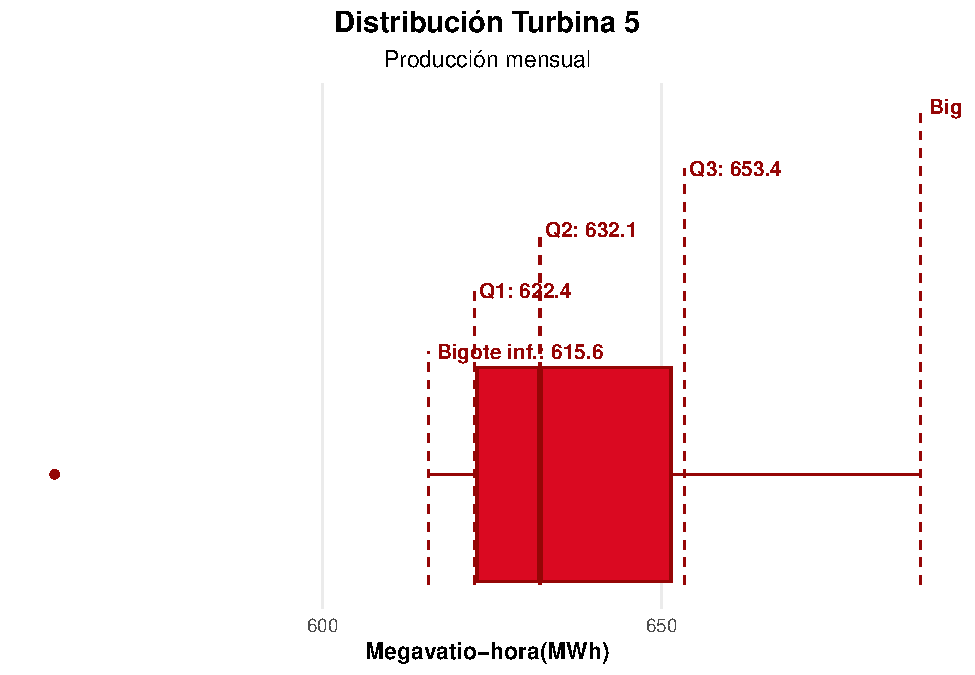
\includegraphics[width=1\linewidth]{Taller-03_files/figure-latex/unnamed-chunk-8-1} \end{center}

\ldots{}

\ldots{}

\noindent\textbf{Pregunta 7. Ajuste un modelo de regresión lineal simple para explicar la producción usando la variable de turbina ¿A qué es igual el R2 del modelo ajustado? ¿Cómo interpreta los parámetros estimados del modelo? ¿Cuál es la categoría de referencia pra el modelo ajustado?}

\begin{Shaded}
\begin{Highlighting}[]
\CommentTok{\# Cambiar el formato de los datos de ancho a largo}

\NormalTok{datos22 }\OtherTok{\textless{}{-}} \FunctionTok{pivot\_longer}\NormalTok{(datos2, }\AttributeTok{cols=}\FunctionTok{c}\NormalTok{(T1,T2,T3,T4,T5),}
                        \AttributeTok{names\_to=}\StringTok{\textquotesingle{}Turbina\textquotesingle{}}\NormalTok{,}
                        \AttributeTok{values\_to=}\StringTok{\textquotesingle{}Producción\_Mensual\_Promedio\textquotesingle{}}\NormalTok{)}
\end{Highlighting}
\end{Shaded}

\begin{Shaded}
\begin{Highlighting}[]
\NormalTok{reg }\OtherTok{\textless{}{-}} \FunctionTok{lm}\NormalTok{(Producción\_Mensual\_Promedio }\SpecialCharTok{\textasciitilde{}}\NormalTok{ Turbina, }\AttributeTok{data =}\NormalTok{ datos22)}
\FunctionTok{summary}\NormalTok{(reg)}
\end{Highlighting}
\end{Shaded}

\begin{verbatim}
## 
## Call:
## lm(formula = Producción_Mensual_Promedio ~ Turbina, data = datos22)
## 
## Residuals:
##    Min     1Q Median     3Q    Max 
## -77.95 -20.36  -3.83  26.50  93.77 
## 
## Coefficients:
##             Estimate Std. Error t value Pr(>|t|)    
## (Intercept) 633.0908    11.1158  56.954   <2e-16 ***
## TurbinaT2   -16.9046    15.7201  -1.075    0.287    
## TurbinaT3    -0.4173    15.7201  -0.027    0.979    
## TurbinaT4   -11.4873    15.7201  -0.731    0.468    
## TurbinaT5     2.0254    15.7201   0.129    0.898    
## ---
## Signif. codes:  0 '***' 0.001 '**' 0.01 '*' 0.05 '.' 0.1 ' ' 1
## 
## Residual standard error: 38.51 on 55 degrees of freedom
## Multiple R-squared:  0.03937,    Adjusted R-squared:  -0.03049 
## F-statistic: 0.5635 on 4 and 55 DF,  p-value: 0.6901
\end{verbatim}

\ldots{}

\noindent\textbf{Pregunta 8. Mediante los parámetros del modelo ajustado, ¿cuál es la producción promedio de la turbina 4? verifique el resultado calculando el promedio simple para las observaciones de la turbina en cuestión.}

\ldots{}

\noindent\textbf{Pregunta 9. Determine mediante una prueba estadística apropiada si existen diferencias significativas entre la producción promedio de energía de las turbinas. ¿A qué es igual el valor del estadístico F en la prueba de hipótesis correspondiente?}

\ldots{}

\noindent\textbf{Pregunta 10. Encuentre los residuales del modelo ajustado y con estos realice una estimación kernel de la densidad (como lo vimos en la primera sesión de clase) junto a un histograma. ¿Encuentra una distribución conocida para los residuales del modelo?}

\ldots{}

\end{document}
